\documentclass{../source/Experiment}

\major{信息工程}
\name{姚桂涛}
\title{神经网络简介}
\stuid{3190105597}
\college{信息与电子工程学院}
\date{\today}
\lab{教11-400}
\course{人工智能实验}
\instructor{胡浩基、魏准}
\grades{}
\expname{神经网络简介}
\exptype{设计验证}
\partner{}
\begin{document}
    \makecover
    \section{实验题目}
        \subsection{实验5-1}
        通过SGD训练方法及Delta 规则,对上述神经
        网络进行训练,并输出训练后的结果。
        
        通过Batch训练方法及Delta 规则,对上述神经
        网络进行训练,并输出训练后的结果。
        
        比较SGD训练方法及Batch训练方法误差(真实
        结果与输出的MSE)随epoch变化趋势,并可视
        化结果

    \section{实验代码}
    \subsection{LPP.py}
    \lstinputlisting[
        language  =   Python
        ]{./Part5/5-1.py}
   

    \section{实验结果}
        \subsection{实验5-1}
            可视化结果
            \begin{figure}[H]
                \centering
                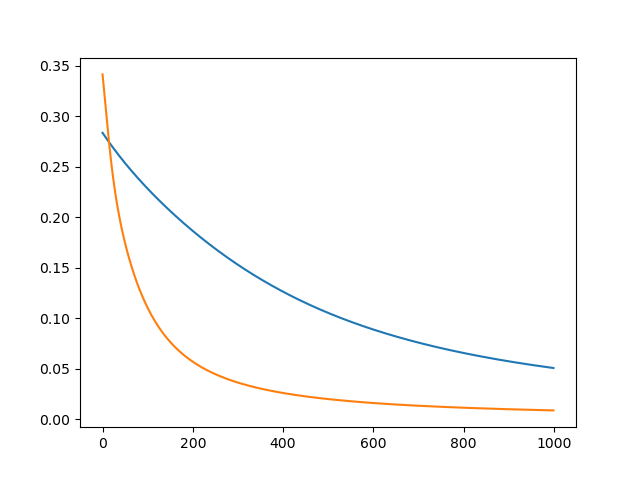
\includegraphics[width = 0.6\textwidth]{Part5/5-1.png}
                \caption{可视化}
            \end{figure}

\end{document}


